\chapter{Run-to-run variance, statistical power, and paired comparisons}
\label{ch01-variance-power-paired-comparisons}
\section{One run is one draw}\label{one-run-is-one-draw}

I created an evaluation tool called CodeProbe (\href{https://github.com/sjarmak/codeprobe}{public repository}) that mines tasks from a repository's merged pull requests. In one of my runs using the tool it had reported that one configuration led another by +0.054 on a task family, and a single task accounted for most of that gap with a +0.300 advantage. This seemed reasonable, nothing about the run was `wrong', and the scoring code returned a number precise to three decimal places. I could easily have written the larger score up as a win.

But, in my stubborn scientific ways, I reran the family instead, three times per configuration. The difference fell to +0.0035, with a 95\% \textbf{confidence interval}, the range produced by a procedure that covers the true value in 95\% of repeated experiments, running from -0.0005 to +0.0074. The five tasks in the family were the paired units: the three repeats collapsed into one per-configuration score for each task, leaving five paired observations and 4 degrees of freedom. The paired t statistic of 2.41 fell below the critical value of 2.776, so the result was the semi-dreaded `not significant'. The task that had appeared to improve by +0.300 came back at exactly 0.000, with both configurations scoring 0.800 on every repeat.

Those reruns showed that the original observation could not justify a claim that would have been easy to make. One bad baseline score created the outlier, and the outlier disappeared once the trial was repeated. Three decimal places of `precision' is meaningless with a single run, and it describes the format of the number while indicating nothing about the stability of the process that produced it.

This task family scores through a deterministic test-suite oracle, under which the end state either passes the fixed tests or does not. That oracle collapses different trajectories onto the same score, so the tight repeat scores are a certification of scorer stability rather than agent determinism. The conclusion covers these five fixed tasks and no wider population.

It is critical to record repeated independent runs before declaring a meaningful difference between agent systems. A single score is one outcome from a variable execution process, even when the configuration appears deterministic. Without repeats, the observed difference mixes the system change I intended to test with variation from model execution, infrastructure, task ordering, and the other choices built into the evaluation apparatus.

Agent evaluations usually arrive as a table with one row per system and one score per row, which suppresses the execution history behind each cell. A score can aggregate hundreds of tasks and still be a single run, if each task was attempted once under one instantiation of the surrounding conditions.

Each cell has three layers behind it. A public agent benchmark is a shared, published task suite used to score agents: \textbf{SWE-bench} presents real issues from software repositories, and tests decide whether a proposed change passes or fails, with SWE-bench Verified as a human-screened subset of those tasks. The \textbf{evaluation harness} is the execution and scoring apparatus that checks out the repository, supplies the task, invokes the agent, applies its change, runs the tests, and produces the reported number. The published comparison is the third layer, assembled from many harness executions.

Repeated attempts need their own vocabulary. \textbf{\href{mailto:pass@k}{\nolinkurl{pass@k}}} names success across repeated attempts: \href{mailto:pass@1}{\nolinkurl{pass@1}} is the fraction of tasks solved in one attempt, \href{mailto:pass@k}{\nolinkurl{pass@k}} is the probability that at least one of k attempts passes, and pass\textsuperscript{k} the probability that all k attempts pass. One opportunity, retries available, and consistency across every attempt are three different questions. A run-level record keeps them separable by storing each attempt's outcome next to its task identity, and an item-level record joins those attempts back to the task. An aggregate is the summary computed from those records; a distribution is the set of outcomes before that aggregation.

Large-scale measurement shows how much of that hidden history reaches the score. Across 60,000 SWE-bench-Verified trajectories, single-run \href{mailto:pass@1}{\nolinkurl{pass@1}} varied by 2.2 to 6.0 percentage points. At decoding temperature 0, where temperature controls how randomly the model selects each token, the standard deviation still exceeded 1.5 percentage points because of infrastructure nondeterminism. The trajectories began to diverge within the first few percent of generated tokens, and each difference changed the context for the next token, so the divergence cascaded through the run.

Temperature 0 therefore does not deliver a deterministic code-generation evaluation. Ouyang et al.~(\href{https://arxiv.org/abs/2308.02828}{2023}) reached the same qualitative conclusion in an earlier empirical study of code generation: nominally identical requests produced different programs and different outcomes. That variation was not confined to the sampling control the model API exposes.

These findings influence how I read benchmark evaluation claims. Improvements of 2 to 3 percentage points, a common magnitude in system comparisons, fit inside the single-run variation Bjarnason et al.~(\href{https://arxiv.org/abs/2602.07150}{2026}) observed across 60,000 trajectories. That envelope applies to SWE-bench-Verified-class tasks, models, and execution conditions, but it is not a universal constant, and it is necessary to estimate local spread before treating a delta of that size as an improvement.

A small p-value also does not repair a single-score comparison. Reimers and Gurevych (\href{https://arxiv.org/abs/1803.09578}{2018}) compared one score from each of two identical systems and found apparent significant differences in up to 26\% of comparisons at p \textless{} 0.05. The test correctly described the two observed runs, but it could not establish that the methods differed, because the experiment had not sampled enough runs to estimate method-level variation.

Seed choice exposes the same failure at a different layer. Two five-seed samples from the same algorithm can look as if they came from different distributions. In reinforcement-learning experiments, Henderson et al.~(\href{https://arxiv.org/abs/1709.06560}{2017}) found that unreported choices among seeds, environments, and evaluation checkpoints gave researchers enough degrees of freedom to promote an ordinary fluctuation into a state-of-the-art claim. Selecting the best run after inspecting the results performs the same transformation more insidiously.

The history predates current agents. Across 2,100 trials that fine-tuned BERT models at identical hyperparameters, Dodge et al.~(\href{https://arxiv.org/abs/2002.06305}{2020}) found that distinct seeds produced substantially different results, and that weight initialization and data order contributed comparable variation. That result concerns small-data fine-tuning of pretrained encoders, so it needs re-verification before anyone treats it as a measured property of large-scale instruction tuning. What it establishes today is that a fixed hyperparameter record can leave consequential experimental state unspecified.

Nuisance sources, e.g., factors that affect the measured result but are not the capability under evaluation, are better varied by design than left to accident. Seeds, data order, task order, and splits can all be randomized, and the corresponding realizations can be matched across the systems being compared. Bouthillier et al.~(\href{https://arxiv.org/abs/2103.03098}{2021}) found that randomizing many nuisance sources and averaging the results approximated the estimator obtained by controlling each source, at about 51 times less compute. Fixed seeds produced precise estimates conditional on one arbitrary configuration, rather than estimates averaged over the range of configurations the benchmark was meant to represent.

Prompt wording is another nuisance source. In a study spanning 53 mostly classification and few-shot tasks, Sclar et al.~(\href{https://arxiv.org/abs/2310.11324}{2023}) found that meaning-preserving changes in prompt formatting produced a median accuracy spread of 7.5 percentage points, with spreads as large as 76 points. On some tasks, Salinas and Morstatter (\href{https://arxiv.org/abs/2401.03729}{2024}) found that trivial edits changed more than 10 percent of predictions. Mizrahi et al.~(\href{https://arxiv.org/abs/2401.00595}{2024}) found that individual templates even reversed which model appeared to perform better, despite greater stability in aggregate comparisons.

Those results do not establish an equivalent variance rate for long-horizon agents. Prompt phrasing should be treated as a local sensitivity measure. It tells us how much a particular result moves under reasonable reformulations, not how much agent performance varies in general.

Prompt variation also creates an ownership problem. Teams often freeze one prompt and describe the resulting configuration as fixed, even though that wording is only one realization from a broader family of semantically equivalent instructions. Fixing the prompt supports reproducibility. Varying it tests whether the conclusion survives reasonable changes in expression. A credible comparison needs both. The exact prompt should be reported so the experiment can be reconstructed, and prompt sensitivity should be measured whenever the conclusion could plausibly depend on wording.

Repeated runs make these hidden choices visible as a distribution. For each configuration, I report every run-level score, along with the mean and standard deviation across runs, and inspect the per-item outcomes behind those aggregates. I randomize the declared nuisance sources and, wherever the design permits, use the same realizations for both configurations. Reporting only the best run identifies the luckiest draw, not how the configuration performs across draws.

Repetition is a direct cost multiplier. Three runs require roughly three times the model calls and execution capacity of one run, before adding prompt or seed variants. That cost cannot be avoided by borrowing a variance estimate from another model or task suite, because observed variance depends on the model, the tasks, and the evaluation apparatus together. Provider-side updates introduce temporal drift that local repetition cannot remove. Repeated results therefore also require either a pinned model version or an explicit record that the provider does not make one available.

The operational rule is narrow. Measure the local run-to-run spread, and do not credit a difference that remains smaller than that spread. Repetition alone does not establish that a detected difference is large enough to matter, nor does it determine how many runs are sufficient. Both depend on the decision threshold and the statistical power of the experiment.

\section{What could the experiment have detected?}\label{what-could-the-experiment-have-detected}

Before running a suite, the first question is which differences the design can resolve at all. In Miller's worked example (\href{https://arxiv.org/abs/2411.00640}{2024}), sampling more responses per question reduced the minimum detectable effect from 13.2 percent to 7.5 percent. The minimum detectable effect is the smallest difference the experiment can reliably distinguish from noise. Neither the model nor the questions became more accurate. Each question simply produced a less variable estimate, allowing the same experiment to resolve a smaller difference.

I run a \textbf{power analysis} before commissioning an evaluation. The calculation relates sample size, variance, the false-positive rate, and the probability of detecting a specified difference. I set that difference to the smallest change that would alter the engineering decision, not the difference I hope to report. This prior \textbf{effect size} is the magnitude assumed before any results are observed.

Statistical and engineering importance must be separated during design. An experiment sized to detect a gain too small to justify a more expensive configuration spends capacity on a decision that will never be made. The target should therefore be the smallest improvement that would justify deployment. Writing that threshold down before the results arrive prevents the observed delta from redefining what counts as a win.

Power is the probability that an experiment detects the specified effect when that effect is present. The false-positive rate controls how often the test reports a difference when no difference exists under its assumptions. These error controls trade off through sample size. At a fixed variance, a smaller target effect, a lower false-positive rate, or a higher desired detection probability each increases the number of observations required.

The minimum detectable effect expresses the same power calculation in reverse. Fix the task set, repeat count, variance estimate, and error rates, and it states the experiment's resolution. Reporting it clarifies what a null result can support. The experiment had adequate power to detect differences of that magnitude or larger, while smaller differences were not reliably distinguishable from noise.

Many published benchmark comparisons cannot support the distinctions their tables imply. In a power analysis of GLUE, Card et al.~(\href{https://arxiv.org/abs/2010.06595}{2020}) found that many test sets lacked the resolution needed to distinguish the small state-of-the-art improvements researchers reported. This does not mean every reported ordering was false. It means the available samples left too much uncertainty to establish those differences at the chosen error rates.

An underpowered study fails in two directions. Most real effects will not reach significance, filling the literature or internal decision record with inconclusive null results. Among the estimates that do cross the significance threshold, the observed effects tend to be exaggerated because unusually large estimates are the ones most likely to survive. A significant result from a weak experiment can therefore provide a much less reliable estimate of magnitude than its p-value suggests.

I estimate the required sample size from a pilot and then add margin. The pilot supplies a variance estimate for the planned model, task family, prompts, and evaluation apparatus. Colas, Sigaud and Oudeyer (\href{https://arxiv.org/abs/1806.08295}{2018}) recommend at least 20 pilot runs for estimating this variance. That is a floor for the pilot estimate, not a claim that the estimate has stabilized or that every final configuration requires 20 repetitions. A small or unrepresentative pilot can understate variance and produce a design that appears adequate on paper but remains underpowered in practice.

The sizing sequence remains reproducible even when its inputs change. I choose the smallest effect that would alter the engineering decision, estimate variance from the pilot, set the false-positive rate and desired detection probability, and solve for the required item and run counts. At fixed error rates, greater variance increases the required sample size, while a larger target effect reduces it. For a suite whose counts are already fixed, I solve in the other direction for the minimum detectable effect and add margin for uncertainty in the pilot estimate.

Which count to increase depends on where the uncertainty originates. More benchmark items reduce uncertainty about performance across items. More independent runs reduce uncertainty from execution variation. More responses per question reduce answer-level variance. Holding the other design choices constant, additional responses cost more model calls but can allow the experiment to resolve a smaller difference.

This is what reduced the minimum detectable effect from 13.2 percent to 7.5 percent in the worked example. The three counts are not interchangeable because each averages over a different random quantity. That measured reduction is one empirical result, not a general conversion between response count and experimental resolution.

Lowering temperature is not a substitute for sampling more responses when the deployed system will run at the original temperature. It changes the distribution being measured rather than estimating that distribution more precisely. A lower temperature is a legitimate system change when the deployed configuration will use it, but it cannot serve as free variance reduction in an experiment intended to evaluate another configuration.

Small run counts also affect which inferential procedure is defensible. A \textbf{bootstrap} estimates uncertainty by resampling the observed data. In a paired comparison, it resamples the observed pairs. In experiments on reinforcement-learning systems, Colas et al.~(2018) found that the bootstrap produced a realized false-positive rate of about 10 percent at small sample sizes despite a nominal rate of 5 percent. Two identical implementations of DDPG, a continuous-control reinforcement-learning algorithm, also appeared significantly different when evaluated with only five runs. Under those measured conditions, Welch's t-test performed better than the bootstrap, and the evidence supported using a false-positive threshold below 0.05.

Welch's t-test does not assume that the two configurations have equal variance, which makes it a more defensible default than the equal-variance t-test for independent small samples. Its advantage at low run counts is empirical and conditional. When the design pairs observations across matched tasks or nuisance realizations, the analysis should preserve that pairing rather than treat the samples as independent. No test removes the need to inspect the score distribution, and no test can repair samples that fail to represent the intended population.

Standard power formulas often assume that aggregated performance is approximately bell-shaped. Reinforcement-learning outcomes can be strongly bimodal, and agent outcomes may similarly divide between complete success and early failure. In the measured reinforcement-learning cases, even the t-test did not fully control the type I error rate for bimodal outcomes. Analytical power calculations should therefore be treated cautiously when the observed distribution is highly discrete, skewed, or multimodal.

Sizing from pilot tasks also assumes that their variation resembles the evaluation suite and that the suite resembles the deployment workload behind the decision. More runs can narrow uncertainty around the wrong population. No sample-size formula can repair a task distribution that omits important cases the deployed system will encounter.

Retrospective power does not solve these limitations. Computing power from the observed effect reuses the noisy outcome as though it had been the design target. The result largely restates the p-value and creates circular reasoning. A small observed effect produces low reported power, while a large observed effect produces high reported power. The useful calculation happens before the result, using an effect threshold and variance estimate chosen independently of the observed comparison.

One of my evaluation frameworks makes refusal mechanical. It scores a system across a ladder of successively weakened configurations and locates each readout on the resulting score curve. When too few rungs have been evaluated, the grader cannot place the readouts reliably, so it raises an error and emits no verdict. This refusal is a methodological rule, not a statistical test, and it carries no false-positive or false-negative rate of its own. Its value is that it keeps insufficient resolution visible to the person making the engineering decision.

A completed comparison should therefore report its detectable range. When the observed difference falls below the predeclared engineering threshold or below the experiment's minimum detectable effect, I report that limitation explicitly. Insufficient resolution is not evidence that the systems are equal.

\section{Compare outcomes item by item}\label{compare-outcomes-item-by-item}

When two systems face the same tasks, the comparison should be based on their per-item differences, and the experiment must preserve those differences from the start. A \textbf{paired design} runs both systems on the same experimental units so that their outcomes can be compared item by item. Pairing is a property of the experiment. The statistical test is chosen only after the paired observations exist.

The identical-system comparisons discussed earlier show the limit of analyzing one aggregate score from each run. A test may determine whether two realized scores differ under its assumptions, while the scientific question concerns whether the underlying methods differ across repeated realizations. Pairing does not answer that second question. Repeated runs are still needed to estimate variation across realizations. Pairing instead improves precision for the comparison within each realization.

The gain comes from removing shared item difficulty. If both systems tend to succeed on easy tasks and fail on hard ones, their item-level scores will be positively correlated. Subtracting the scores item by item removes much of that common movement, leaving variation that more directly represents disagreement between the systems.

For item \(i\), let \(x_i\) and \(y_i\) be the two system scores and define the paired difference as \(d_i=x_i-y_i\). Across \(n\) items, the estimated mean difference and its standard error are

\[
\bar d=\frac{1}{n}\sum_{i=1}^{n}d_i,
\qquad
SE(\bar d)=\frac{s_d}{\sqrt n}.
\]

The variance of the mean difference contains the covariance between the two systems:

\[
\operatorname{Var}(\bar d)
=\frac{s_x^2+s_y^2-2\operatorname{Cov}(x,y)}{n}.
\]

When the systems respond similarly to item difficulty, the covariance is positive and reduces the variance of the comparison. An independent analysis omits this term. It treats the two systems as though they had been evaluated on unrelated samples and counts the variation between easy and hard tasks twice. The resulting uncertainty estimate is therefore unnecessarily large when item-level outcomes move together.

\begin{figure}[htbp]
\centering
\pandocbounded{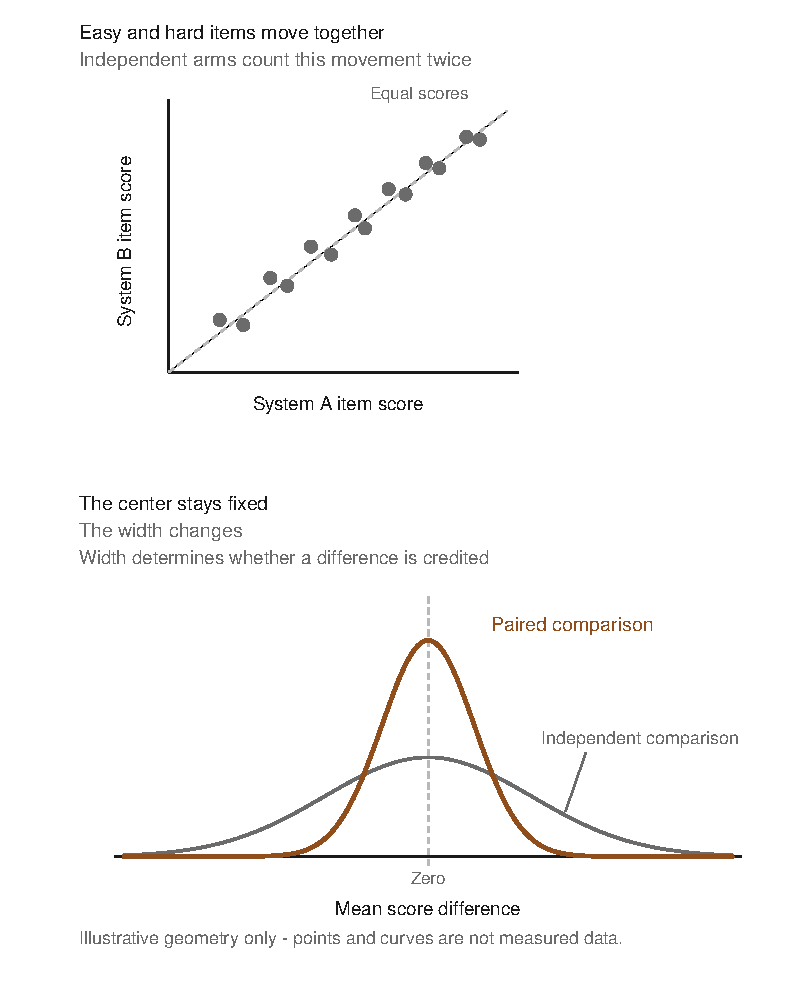
\includegraphics[keepaspectratio,alt={Illustrative, unmeasured geometry shows item scores for systems A and B rising together, while paired and independent mean-difference distributions share zero but pairing produces narrower uncertainty.}]{figures/ch01-paired-comparison.pdf}}
\caption{Illustrative, unmeasured geometry shows item scores for systems A and B rising together, while paired and independent mean-difference distributions share zero but pairing produces narrower uncertainty.}
\end{figure}

Item-level subtraction removes shared task difficulty, so the remaining variation better represents system disagreement. Positive covariance narrows uncertainty without changing the mean difference.

The interval around the mean difference is obtained by multiplying its standard error by an appropriate critical value. The choice of critical value and the validity of the approximation depend on the statistical procedure and the observed score distribution.

The data record must preserve the pairing. For every task, I retain the task identity, both system scores, the nuisance-source assignments, and the run identity. I report the mean paired difference, its standard error, an interval around that mean, and the correlation between the systems' item-level scores. Once the per-item relationship has been discarded, two headline means are not enough to reconstruct any of these quantities.

Pairing also improves diagnosis. The same average difference can arise from small gains across most tasks, a few large reversals, or a trade in which each system solves a different subset. Those patterns have different engineering implications. Item-level records reveal which tasks changed and whether the overall result depends on a small number of discordant cases.

The validity of the pairing depends on experimental identity, not matching task labels. Both systems must receive the same task state under the same execution and scoring apparatus. Repository revision, dependency state, tool permissions, time limits, and scoring logic are all part of the experimental unit. If any of them differ between the two arms, the subtraction no longer removes shared task difficulty because the systems did not receive the same item.

An adversarial review of one of my own experiment designs found this exact defect. One arm transformed the repository before presenting it to the system, while the other operated on the original repository. The task label remained the same, but the executable state did not. I therefore treated the planned pairing as invalid. A shared label does not establish that two experimental units are equivalent.

Published aggregate scores create a simpler boundary. If I did not run the other system on the same item instances, I do not have paired observations. The aggregate results can still be compared descriptively, but their item-level covariance cannot be recovered from the means. A valid paired analysis requires rerunning both systems on the same items.

Repeated attempts introduce the same identity requirement. Attempt one from system A pairs with attempt one from system B only when the attempts share randomized conditions by construction. Selecting pairs after inspecting the outcomes biases the comparison. Seeds, task order, data order, and other nuisance assignments must therefore be matched before results are visible and recorded with every pair.

The statistical procedure must also match the mathematical form of the outcome. When the reported score is the arithmetic mean of per-item numerical contributions, and the distribution of paired differences is reasonably compatible with a normal approximation, a paired t-test can test the mean difference and support a corresponding power analysis. That approximation should not be assumed automatically for small, discrete, skewed, or highly irregular samples.

Composite metrics require different treatment. An F-score is a nonlinear function of aggregate counts. There is generally no set of independent per-item F-scores whose arithmetic mean equals the corpus-level F-score. Corpus-level BLEU has a similar aggregation problem, and some forms of ROUGE may also depend on nonlinear or corpus-level aggregation. Applying a t-test to invented per-item metric contributions can produce a familiar p-value without satisfying the mathematical assumptions that give the test meaning.

A paired bootstrap preserves the relationship between the systems by resampling items as pairs and recomputing the full metric on each resampled dataset. A paired permutation test instead exchanges system labels within each observed pair under the null hypothesis. Neither requires the same normal approximation as a parametric t-test. Both still depend on choosing the correct resampling unit and having a sufficiently representative sample. The small-sample bootstrap failure described earlier occurred when the resampling unit was only a handful of runs.

Agent evaluations introduce outcomes that standard benchmark guidance does not fully resolve. Cost-weighted success combines task outcome with resource use. A pass or fail assigned by an imperfect grader includes uncertainty from the grading process. Neither outcome inherits a valid test merely because its final value lies between zero and one. The sampling unit, dependence structure, and aggregation rule must be specified before choosing the analysis.

The table below gives directional guidance. The recommendations for language-generation metrics come from the broader methodological guidance of Dror and Reichart (\href{https://arxiv.org/abs/1809.01448}{2018}) rather than from controlled comparisons of agent evaluations. The binary row applies \textbf{McNemar's test}, introduced by McNemar (\href{https://doi.org/10.1007/BF02295996}{1947}), the standard test for paired pass or fail outcomes. It analyzes the discordant pairs in which one system passes and the other fails. The table is a starting point, not a substitute for deriving the metric's actual sampling structure.

\begin{longtable}[]{@{}
  >{\raggedright\arraybackslash}p{(\linewidth - 4\tabcolsep) * \real{0.3333}}
  >{\raggedright\arraybackslash}p{(\linewidth - 4\tabcolsep) * \real{0.3333}}
  >{\raggedright\arraybackslash}p{(\linewidth - 4\tabcolsep) * \real{0.3333}}@{}}
\toprule\noalign{}
\begin{minipage}[b]{\linewidth}\raggedright
Outcome structure
\end{minipage} & \begin{minipage}[b]{\linewidth}\raggedright
Comparison to analyze
\end{minipage} & \begin{minipage}[b]{\linewidth}\raggedright
Test guidance
\end{minipage} \\
\midrule\noalign{}
\endhead
\bottomrule\noalign{}
\endlastfoot
Per-item numerical scores whose paired differences plausibly satisfy a normal approximation & Mean of the paired item differences & Paired t-test \\
Metrics computed nonlinearly from aggregate counts, including corpus-level F-score and BLEU & Full metric recomputed on resampled or relabeled item pairs & Paired bootstrap or paired permutation test \\
Pass or fail outcomes on the same items & Discordant pairs in which only one system passes & McNemar's test \\
\end{longtable}

A later chapter on retrieval freshness uses McNemar's test for this reason. Both systems receive the same items, and each item produces a pass or fail outcome.

The companion catalog covers designs that this basic framework does not. Clustered items require correlation-aware standard errors. Estimating pass@(k) from repeated attempts requires the appropriate combinatorial estimator. Claims spanning many tasks or metrics require multiplicity correction. Ranking several systems rather than comparing two requires paired-comparison ranking models with uncertainty intervals.

The catalog also covers profiling benchmark noise before making decisions, declaring the decoding configuration, aggregating scarce repetitions with interquartile means and resampled intervals, reducing an evaluation around a specific decision, using precommitted confirmatory designs, and measuring sensitivity across prompt variants. Each addresses a narrower problem than the core decisions developed in this chapter.

\section{Before drawing a conclusion from a difference}\label{before-drawing-a-conclusion-from-a-difference}

I define the engineering threshold before running the expensive suite. The threshold is the smallest change that would alter the engineering decision, not the smallest change a statistical test might detect.

Pilot variance then determines the required numbers of tasks and repeated runs. I add margin because the pilot estimate is itself uncertain, and the design record states the smallest difference the planned experiment can reliably resolve. When the available budget cannot resolve a difference large enough to matter, I narrow the claim or withhold the verdict before spending the calls.

Three independent repeats per configuration are my minimum. Three may still produce an unstable variance estimate, but they prevent one unusually favorable or unfavorable run from determining the result. I pair nuisance conditions across systems wherever possible and run both systems against identical item states. Each retained row records the item identity, the outcomes from both systems, the repeat identity, and the assigned random conditions.

The analysis begins with per-item differences. For continuous outcomes, I report the mean paired difference, its standard error, the correlation between the two systems' scores, and a confidence interval for the mean difference.

Binary pass-or-fail outcomes require the discordant pairs and an appropriate paired test. Nonlinear composite metrics require resampling or permutation of intact pairs. Matching task names do not create a paired design when the repository state, inputs, or execution path differs.

\Needspace{5\baselineskip}

Repeated trials remain interpretable only while the apparatus is pinned:

\begin{itemize}
\tightlist
\item
  model version;
\item
  decoding settings;
\item
  exact prompts;
\item
  task and repository revision;
\item
  tool definitions and permissions;
\item
  harness version; and
\item
  evaluator version.
\end{itemize}

When a provider exposes no stable model version, I record the evaluation window and treat later reruns as potentially affected by model drift.

The observed difference belongs beside the complete run distribution and the engineering threshold written before execution. I do not credit a difference that remains smaller than the measured variation. I return no verdict when the experiment lacked the power to resolve the difference that would have changed the decision.

\section*{Sources and evidence}

The evidence grouping on each entry below comes from its catalog record. Author-system cases in this chapter are narrative illustration and are not part of the evidence base.

\textbf{Never report a single run}

\begin{itemize}
\tightlist
\item
  Strong evidence: Ouyang, Zhang, Harman \& Wang (2023). An Empirical Study of the Non-determinism of ChatGPT in Code Generation. arXiv:2308.02828. Nominally identical requests, different programs and outcomes.
\item
  Strong evidence: Bjarnason, Silva \& Monperrus (2026). On Randomness in Agentic Evals. arXiv:2602.07150. The 60,000-trajectory result: 2.2 to 6.0 pp single-run spread, SD above 1.5 pp at temperature 0, early-token divergence.
\item
  Strong evidence: Reimers \& Gurevych (2018). Why Comparing Single Performance Scores Does Not Allow to Draw Conclusions About Machine Learning Approaches. arXiv:1803.09578. The 26\% result.
\item
  Strong evidence: Bouthillier et al.~(2021). Accounting for Variance in Machine Learning Benchmarks. MLSys 2021. arXiv:2103.03098. The \textasciitilde51x result and the fixed-seed critique.
\item
  Strong evidence: Henderson et al.~(2017). Deep Reinforcement Learning that Matters. AAAI 2018. arXiv:1709.06560. Five-seed splits and unreported researcher degrees of freedom.
\item
  Strong evidence: Dodge et al.~(2020). Fine-Tuning Pretrained Language Models: Weight Initializations, Data Orders, and Early Stopping. arXiv:2002.06305. The 2,100-trial seed result, scoped to small-data fine-tuning of pretrained encoders.
\item
  Prompt-variance finding: incorporated into this chapter's first developed practice, with its full evidence recorded in the companion catalog. Strong evidence: Sclar et al.~(2023), FormatSpread, arXiv:2310.11324; Mizrahi et al.~(2024), TACL, arXiv:2401.00595; and Salinas and Morstatter (2024), arXiv:2401.03729.
\end{itemize}

\textbf{Analyze statistical power before running}

\begin{itemize}
\tightlist
\item
  Strong evidence: Miller (2024). Adding Error Bars to Evals. arXiv:2411.00640 (Anthropic). The 13.2\% to 7.5\% minimum-detectable-effect example and the response-count lever.
\item
  Strong evidence: Card et al.~(2020). With Little Power Comes Great Responsibility. EMNLP 2020. arXiv:2010.06595. GLUE underpowering and effect-size exaggeration.
\item
  Strong evidence: Colas, Sigaud \& Oudeyer (2018). How Many Random Seeds? arXiv:1806.08295. The pilot floor, the bootstrap false-positive rate at small N, the DDPG case, and the preference for Welch's t-test.
\end{itemize}

\textbf{Use paired tests matched to the metric}

\begin{itemize}
\tightlist
\item
  Strong evidence: Miller (2024). Adding Error Bars to Evals. arXiv:2411.00640. Paired per-item differences with paired standard error and score correlation.
\item
  Directional evidence: Dror \& Reichart (2018). Appendix, Recommended Statistical Significance Tests for NLP Tasks. arXiv:1809.01448. The per-metric test selection; directional, so the table is guidance, not a measured result.
\item
  Foundational method: McNemar, Q. (1947). Psychometrika 12(2), 153-157. DOI: 10.1007/BF02295996. The paired pass/fail test used in the binary-outcome row.
\end{itemize}

\textbf{Author-system illustration cited inline}

\begin{itemize}
\tightlist
\item
  Not an evidence item: CodeProbe, the author's task-mining evaluation tool, \href{https://github.com/sjarmak/codeprobe}{public repository}. Named inline for the task-family run and rerun described in the opening, which are narrative illustration.
\end{itemize}
